 %%%%%%%%%%%%%%%%%%%%%%%%%%%%%%%%%%%%%%%%%%%%%%%%%%%%%%%%%%%%%%%%%%%%%%%%%%%%%%%%%%%%%
% ITR_LSR_slides class options
% - 'itr' or 'ITR' for ITR version
% - 'lsr' or 'LSR' for LSR version
% - 'german' for a German presentation
% - 'english' for an English presentation (default)
% - 'longpres' if you want to use subsections
% - 'noshadow' if you want to use blocks without shadow
% - 'draftlayout' to show a mm grid as overlay for precise positioning
% - 'presentermode' to generate slides with note-page, usable with e.g. pympress
% - 'coveredhidden' to hide covered objects. Default is transparent.
% beameroptions can be used, e.g.:
% - 'aspectratio=169' for 16:9 wide screen presentations
% - `handout` to generate printable handout sheets
% - `draft` for fast compilation (without graphics)
% do not remove STUDENT option!
%%%%%%%%%%%%%%%%%%%%%%%%%%%%%%%%%%%%%%%%%%%%%%%%%%%%%%%%%%%%%%%%%%%%%%%%%%%%%%%%%%%%%
\documentclass[student, noshadow, itr, english, aspectratio=169]{ITR_LSR_slides}
\usepackage{tikz}
\usepackage{pgfplots}
\pgfdeclarelayer{background}
\pgfdeclarelayer{nodelayer}
\pgfdeclarelayer{edgelayer}
\pgfdeclarelayer{foreground}
\pgfsetlayers{background,edgelayer,nodelayer,main,foreground}
% robot name for tikz figure
%\newcommand{\RobotName}{$\mathbf{R}$}

\def\CheckAttentionSlide{
    \begin{frame}
        \begin{center}
            {\fontsize{40}{50} \structure{Sorry for your attention}\\}
        \end{center}
    \end{frame}
}

\addbibresource{./refs/mybib.bib}
\graphicspath{{pics/}{logos/}}

\title{Kernel Embedding for Particle Gibbs-Based Optimal Control}
\presenter{L. Hochschwarzer}

\supervisor{R. Lefringhausen}
\typeofpres{Intermediate Report Master‘s Thesis}

\usepackage[bigfiles]{media9} %option bigfiles not needed for xelatex, runs without problems on ubuntu14
%%%%%%%%%%%%%%%%%%%%%%%%%%%%%%%%%%%%%%%%%%%%%%%%%%%%%%%%%%%%%%%%%%%%%%%%%%%%%%%%

\usepackage{empheq}

\usepackage{tikz}
\usepackage{pgfplots}

\pgfplotsset{compat=1.18}
\usetikzlibrary{arrows,shapes,backgrounds,patterns,fadings,decorations,
	positioning,external,arrows.meta,pgfplots.fillbetween, pgfplots.groupplots}

\begin{document}


\begin{frame}
    \titlepage
\end{frame}


\section{Introduction}
\begin{frame}{Motivation}	
\begin{columns}[onlytextwidth, T]
		\begin{column}{.5\textwidth}
			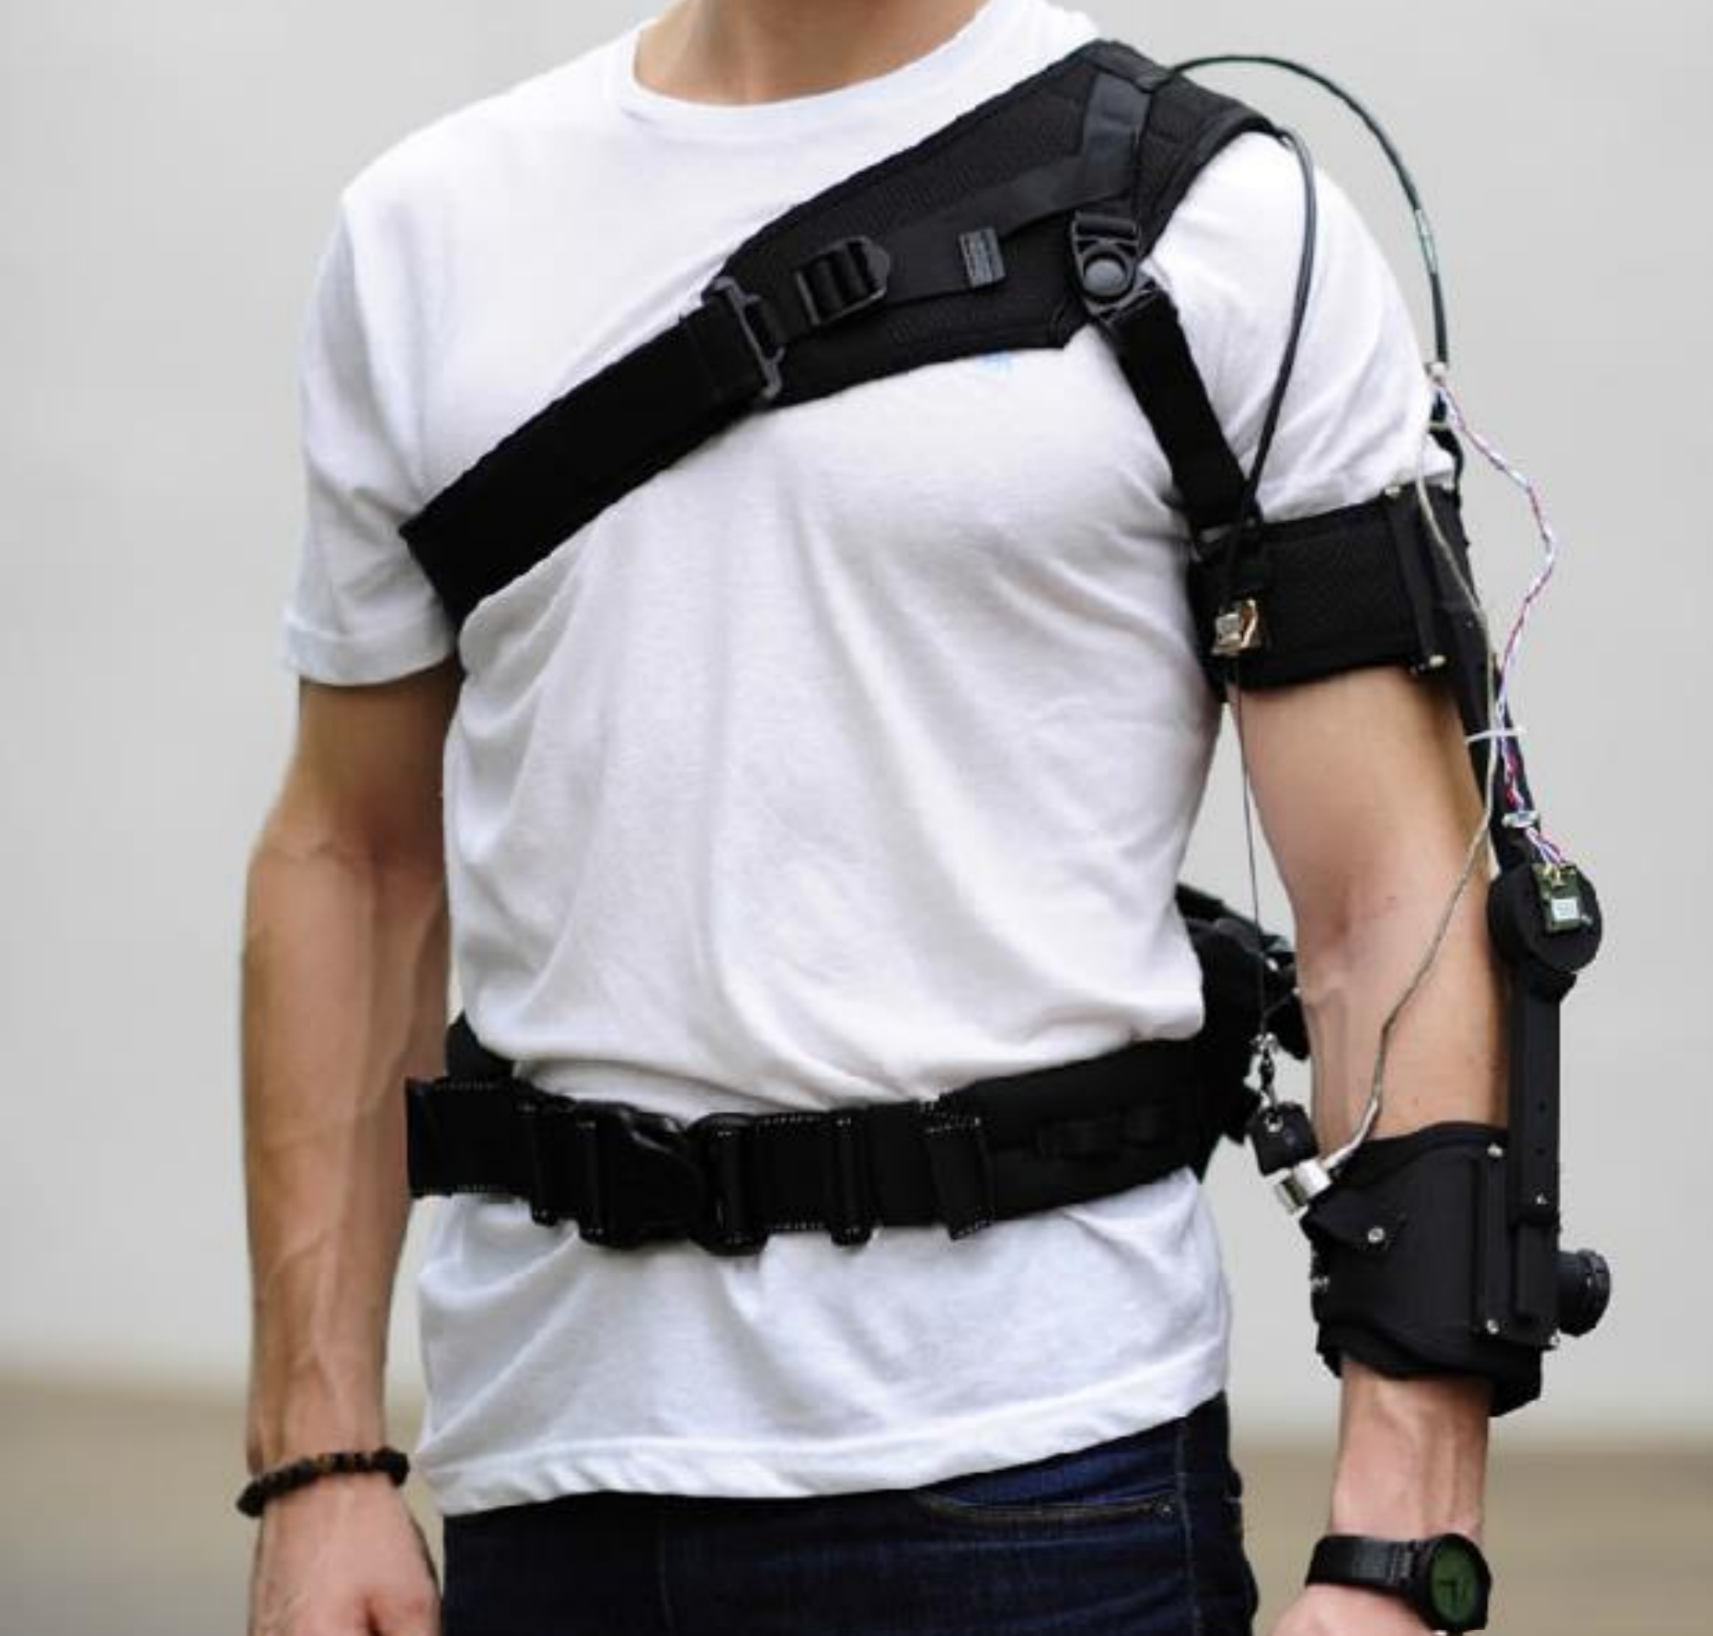
\includegraphics[width= .8\textwidth]{Motivation_pic}
			\cite[4]{Xiloyannis_19}
		\end{column}
		\begin{column}{.5\textwidth}
		\vspace{1cm}
		\textbf{Challenges}:
		\vspace{.2cm}
			\begin{itemize}
			\item Unknown Dynamic
			\item Latent States
			\item Safety
			\end{itemize}
		\end{column}
	\end{columns}\vspace{.5cm}
\end{frame}

\begin{frame}{Problem Statement - System}	
	\textbf{Given:} Dataset $\mathbb{D} = \left\{\boldsymbol{u}_{t}, \boldsymbol{y}_{t}\right\}_{t = \text{-}T:\text{-}1}$ from unknown system
	\begin{equation*}
	\begin{split}
	\boldsymbol{x}_{t+1} &= \boldsymbol{f} \left( \boldsymbol{x}_{t}, \boldsymbol{u}_t \right) + \boldsymbol{v}_{t}, \makebox[1cm]{\hfill} \; \boldsymbol{v}_{t} \sim \boldsymbol{\mathcal{V}},\\
	\boldsymbol{y}_{t} &= \boldsymbol{g} \left( \boldsymbol{x}_{t}, \boldsymbol{u}_t \right) + \boldsymbol{w}_{t}, \makebox[1cm]{\hfill} \boldsymbol{w}_{t} \sim \boldsymbol{\mathcal{W}}
	\end{split}
	\end{equation*}

	\begin{block}{Assumptions}
	\begin{itemize}
		\item 
		Known system structure
	\begin{equation*}
	\begin{split}
	\boldsymbol{x}_{t+1} &= \boldsymbol{f}_{\boldsymbol{\theta}} \left( \boldsymbol{x}_{t}, \boldsymbol{u}_t \right) + \boldsymbol{v}_{t}, \makebox[1cm]{\hfill} \; \boldsymbol{v}_{t} \sim \boldsymbol{\mathcal{V}}_{\boldsymbol{\theta}},\\
	\boldsymbol{y}_{t} &= \boldsymbol{g}_{\boldsymbol{\theta}} \left( \boldsymbol{x}_{t}, \boldsymbol{u}_t \right) + \boldsymbol{w}_{t}, \makebox[1cm]{\hfill} \boldsymbol{w}_{t} \sim \boldsymbol{\mathcal{W}}_{\boldsymbol{\theta}}.
	\end{split}
	\end{equation*}
	\item 
	Known priors $p(\boldsymbol{\theta})$ and $p(\boldsymbol{x}_{\text{-}T})$
	\end{itemize}
	\end{block}	


\end{frame}

\begin{frame}{Problem Statement - Optimal Control Problem}	
	\textbf{Goal:} Solve optimal control problem (OCP)\\
	\begin{block}{Stochastic OCP}
		\begin{equation*}
		\min\limits_{\boldsymbol{u}_{0:H}} J_H(\boldsymbol{u}_{0:H}) 
		\end{equation*}
		subject to: 
		\begin{equation*}
		P \left[ h_i(\boldsymbol{u}_{0:H},  \boldsymbol{x}_{0:H},  \boldsymbol{y}_{0:H}) \leq 0 \right] \geq 1 - \alpha, \; \forall i = 1,...,n_c
		\end{equation*}
	\end{block}	
	\textbf{Problem:} Underlying data distribution $P$ is unknown
\end{frame}

\begin{frame}{Related Works}

Particle Gibbs Based Optimal Control \textbf{\cite[4]{Robert_24}}

$\;\; \Rightarrow \;$ Guarantees determined retroactively

\vspace{.4cm}

Alternative Approaches:
\begin{itemize}
\item Wasserstein Ambiguity \cite[4]{Hota_19}

$\;\; \Rightarrow \;$ Constraints limited to affine functions
\item \makebox[3cm]{ Kernel Embeddings \hfill} \textbf{\cite[4]{Yassine_22}}\\
\makebox[3cm]{\hfill}   \cite[4]{Adam_22} 
\end{itemize}
\end{frame}


\section{Particle Gibbs}

\begin{frame}{Particle Gibbs Scenarios}
Particle Gibbs gives us the scenarios $\boldsymbol{\delta}^{[1:N]} = \{ \boldsymbol{\theta}, \boldsymbol{x}_0, \boldsymbol{v}_{0:H}, \boldsymbol{w}_{0:H}\}^{[1:N]}$ that characterize the system\\

\textbf{Goal:} Reformulate chance-constraint problem with scenarios $\boldsymbol{\delta}^{[1:N]}$

\begin{block}{Chance Constraints}
	\begin{equation*}
		P \left[ h_i(\boldsymbol{u}_{0:H},  \boldsymbol{x}_{0:H},  \boldsymbol{y}_{0:H}) \leq 0 \right] \geq 1 - \alpha, \; \forall i = 1,...,n_c
	\end{equation*}
\end{block}	

\makebox[6.7cm]{\hfill} $\boldsymbol{\Downarrow}$ 

\begin{block}{Scenario Approach (used in \cite{Robert_24})}
	\begin{equation*}
		 \boldsymbol{h}(\boldsymbol{u}_{0:H},  \boldsymbol{x}_{0:H}^{[n]},  \boldsymbol{y}_{0:H}^{[n]}) \leq 0, \; \forall n = 1, ..., N
	\end{equation*}
\end{block}

$\;\; \Rightarrow \;$ Risk factor $\alpha$ not considered in optimization




\end{frame}


\section{Kernel Embedding}

\begin{frame}
	\frametitle{Maximum Mean Discrepancy (MMD) ambiguity sets}
\textbf{Goal:} Reformulate chance-constraint problem with scenarios $\boldsymbol{\delta}^{[1:N]}$\\
\textbf{Idea:} Replace distribution $P$ with the ambiguity set $\mathcal{P}$\\

\begin{columns}[onlytextwidth, T]
\begin{column}{.65\textwidth}

\begin{block}{MMD ambiguity set}
\begin{equation*}
\mathcal{P} =  \left\{ \tilde{P} : \text{MMD} (\tilde{P}, P_N) \leq \varepsilon \right\}.
\end{equation*}
\end{block}	

\makebox[4.2cm]{\hfill} $\boldsymbol{\Downarrow}$ 

\begin{block}{Expanded Chance-Constraints}
\begin{equation*}
\inf\limits_{\tilde{P} \in \mathcal{P}}\tilde{P} \left[ h_i(\boldsymbol{u}_{0:H},  \boldsymbol{x}_{0:H},  \boldsymbol{y}_{0:H}) \leq 0 \right] \geq 1 - \alpha.
\end{equation*}
\end{block}
\end{column}
\begin{column}{.3\textwidth}
\vspace{.5cm}
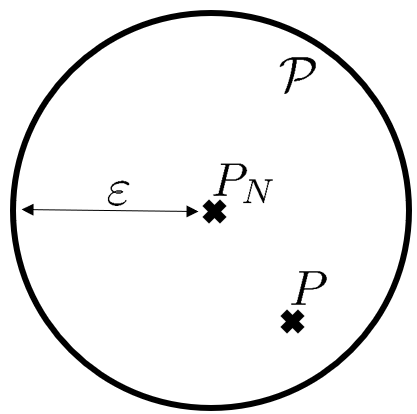
\includegraphics[width= \textwidth]{AmbiguitySetDrawing}
\end{column}
\end{columns}
%With large enough $N \Rightarrow$ $P$ is an element of $\mathcal{P}$

\end{frame}

\begin{frame}
	\frametitle{Constraint Reformulation}
\textbf{Goal:} Reformulate chance-constraint problem with scenarios $\boldsymbol{\delta}^{[1:N]}$
\begin{block}{Feasible Region of chance constraint}
\begin{equation*}
Z_i :=  \left\{ \boldsymbol{u}_{0:H} \in \mathcal{U}^{H+1} : \inf\limits_{\tilde{P} \in \mathcal{P}}\tilde{P} \left[ \tilde{h}_i(\boldsymbol{u}_{0:H},  \boldsymbol{\delta}) \leq 0 \right] \geq 1 - \alpha \right\}
\end{equation*}
\end{block}	

\makebox[6.7cm]{\hfill} $\boldsymbol{\Downarrow}$ 

\begin{block}{Reformulated Feasible Region \cite{Yassine_22}}
\begin{empheq}[right = \empheqrbrace, left= Z_i \coloneqq \empheqlbrace \boldsymbol{u}_{0:H} \in \mathcal{U}^{H+1} :]{align*}
    & g_0 + \frac{1}{N}\sum_{n = 1}^N (\boldsymbol{K}\boldsymbol{\gamma})_n + \varepsilon \sqrt{\boldsymbol{\gamma}^\text{T}\boldsymbol{K}\boldsymbol{\gamma}} \leq t' \alpha \\
    & [\tilde{h}_i(\boldsymbol{u}_{0:H},  \boldsymbol{\delta}^{[n]}) + t']_+ \leq g_0 + (\boldsymbol{K}\boldsymbol{\gamma})_n, \; n = 0,...,N \\
    & g_0 \in \mathbb{R}, \boldsymbol{\gamma} \in \mathbb{R}^N, t' \in \mathbb{R}
  \end{empheq}
\end{block}
\end{frame}


\begin{frame}
	\frametitle{Problem Formulation}
\textbf{Goal:} Reformulate chance-constraint problem with scenarios $\boldsymbol{\delta}^{[1:N]}$
\begin{align*} 
 &\min\limits_{\boldsymbol{u}_{0:H}, \{g_0, \boldsymbol{\gamma}, t'\}^{[1:n_c]}} J_H(\boldsymbol{u}_{0:H}) \\
\text{subject to:}&\; \forall n \in \mathbb{N}_{\leq N}, \;  \forall t \in \mathbb{N}_{\leq H}^0, \; \forall i \in \mathbb{N}_{\leq n_c}  \\
&\left. 
\begin {aligned}
\boldsymbol{x}_{t+1}^{[n]} = \boldsymbol{f}_{\boldsymbol{\theta}^{[n]}} \left( \boldsymbol{x}_{t}^{[n]} , \boldsymbol{u}_t \right) + & \boldsymbol{v}_{t}^{[n]}\\
\boldsymbol{y}_{t}^{[n]} = \boldsymbol{g}_{\boldsymbol{\theta}^{[n]}} \left( \boldsymbol{x}_{t}^{[n]}, \boldsymbol{u}_t \right) + & \boldsymbol{w}_{t}^{[n]} 
\end{aligned}
 \;\;  \right\} \; \text{Dynamic Constraints} \\
&\;\;\;\; \boldsymbol{u}_{0:H} \in Z_i(g_0^{[i]}, \boldsymbol{\gamma}^{[i]}, t'^{[i]}) \;\;\;\;\;\; \;\;\;  \Bigl\} \; \text{Reformulated Chance Constraints}
\end{align*}



\end{frame}

\section{Simulation}

\begin{frame}{Simulation Setup}
\begin{itemize}
\item 
\makebox[4cm]{Unknown system: \hfill}
$\boldsymbol{f}(\boldsymbol{x}, u) = 
\begin{bmatrix}
0.8  x_1 - 0.5 x_2 \\
0.4 x_1 + 0.5 x_2 + u
\end{bmatrix}$ \\
\makebox[4cm]{\hfill} $\boldsymbol{v}_t \sim \mathcal{N} \left(\boldsymbol{0}, \boldsymbol{Q} =  
\begin{bmatrix}
0.03 & \text{-}0.004 \\
\text{-}0.004 & 0.01
\end{bmatrix}
\right).$

\item 
\makebox[4.5cm]{Known system structure: \hfill} $\boldsymbol{f}(\boldsymbol{x}, u) = \boldsymbol{A} \left[ x_1,  x_2,  u \right]^\text{T} + \boldsymbol{v}_{t}, \; \boldsymbol{v}_{t} \sim \mathcal{N} (\boldsymbol{0}, \boldsymbol{Q})$ 
\item
\makebox[4.5cm]{Priors: \hfill} $\boldsymbol{Q} \sim \mathcal{IW} (100 \boldsymbol{I}_2, 10)$ \\
\makebox[4.5cm]{\hfill} $\boldsymbol{A} \sim \mathcal{MN} (\boldsymbol{0}, \boldsymbol{Q}, 10 \boldsymbol{I}_2)\;\;\;\;\;\;\;\;\;\;\;\;\;\;\;\;\;\;$ \cite{Svensson_17}\\
\makebox[4.5cm]{\hfill} $\boldsymbol{x}_{\text{-}T} \sim \mathcal{N} ([2, 2]^\text{T}, \boldsymbol{I}_2)$


\item Known measurement model $g(\boldsymbol{x}, u) = x_1, \; w_t \sim \mathcal{N} (0, 0.1)$

\item Cost function $J_H = \sum_{t = 0}^H u_t^2$

\item Input constraints $\left| u \right| \leq 10$

\item Gaussian kernels with bandwidth $\sigma$ set via the median heuristic \cite{Damien_18}

\item Ambiguity set radius $\varepsilon$ set via bootstrap construction \cite{Yassine_22}.
\end{itemize}
\end{frame}	

\begin{frame}{Optimal Control with Constrained Outputs}

Number of scenarios used for optimization: $N = 200$
\vspace{.3cm}
\begin{columns}[onlytextwidth, T]
		\begin{column}{.5\textwidth}
			\;\; Scenario Approach
			\begin{figure}
			\pgfplotsset{width=\textwidth, compat = 1.18, 
			height = .8\textwidth, grid= major, 
			ticklabel style = {font=\scriptsize},
			every axis label/.append style={font=\scriptsize},
	        }
			\def\file{data/Scenario_K200_S2.txt}
			
			\centering
			\begin{tikzpicture}
			\begin{axis}[
			grid=none,
			xmin=0, xmax=40,
			ymin=-14, ymax=14,
			xtick={0, 10, 20, 30, 40},
			ytick={-10, -5, 0, 5, 10},
			ylabel=$y$, xlabel=$t$,
			set layers=standard]
			
			\addplot[name path=A, forget plot, thick, opacity=0.2] table[x=t,y=y_opt_max]{\file};
			\addplot[name path=B, thick, opacity=0.2] table[x=t,y=y_opt_min]{\file};
			\tikzfillbetween[of=A and B]{opacity=0.2};
			%\addlegendentry{$\left\{y_{0:H}^{[1:N]} \right\}$}
			
			\addplot[ultra thick,black!20!green] table[x=t,y=y_pred]{\file};
			%\addlegendentry{$\frac{1}{N}\sum\limits_{n=1}^N y_{0:H}^{[n]}$}
			
			\addplot[ultra thick, blue] table[x=t,y=y_true]{\file};
			%\addlegendentry{$y_{0:H}$}
			
			\draw [fill=red, fill opacity=0.2,red, opacity=0.2] (10,15) rectangle (20,-10); 
			\draw [fill=red, fill opacity=0.2,red, opacity=0.2] (30,10) rectangle (40,-15); 
			\end{axis}
			\end{tikzpicture}
			\end{figure}
			%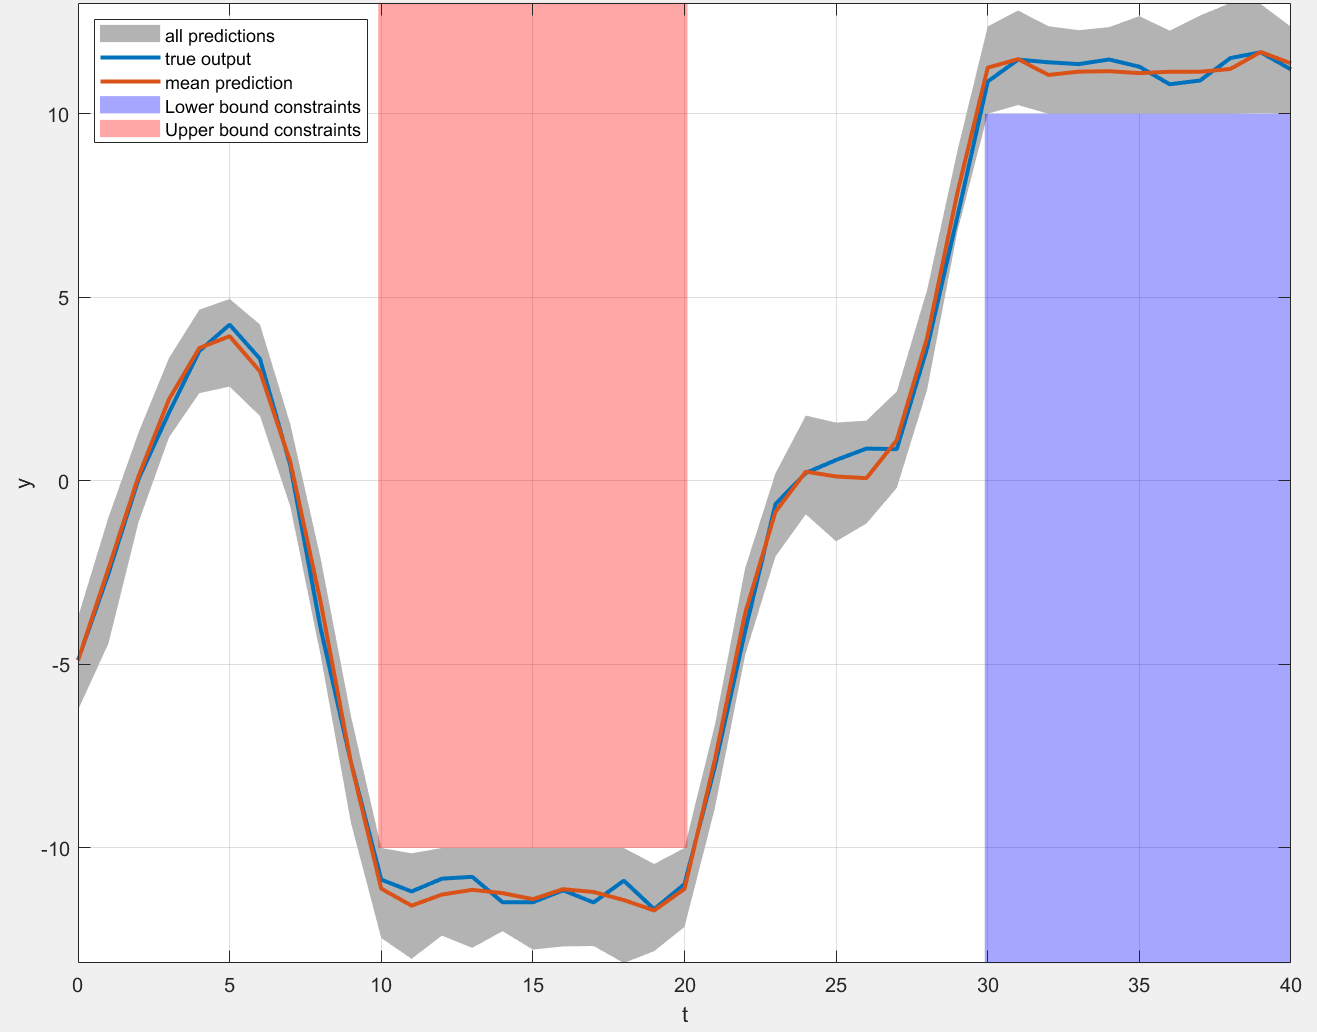
\includegraphics[width= .9\textwidth]{Scenario_plot}
		\end{column}
		\begin{column}{.5\textwidth}
			\only<1>{$\;\;$ Kernel Approach  ($\alpha = 0.1$)
			\begin{figure}
			\pgfplotsset{width=\textwidth, compat = 1.18, 
			height = .8\textwidth, grid= major, 
			legend cell align = left, ticklabel style = {font=\scriptsize},
			every axis label/.append style={font=\scriptsize},
			legend style = {font=\scriptsize},
	        }
			\def\file{data/Kernel_K200_Alpha01_S2.txt}
			
			\centering
			\begin{tikzpicture}
			\begin{axis}[
			grid=none,
			xmin=0, xmax=40,
			ymin=-14, ymax=14,
			xtick={0, 10, 20, 30, 40},
			ytick={-10, -5, 0, 5, 10},
			%ylabel=$y$, 
			xlabel=$t$,
			set layers=standard,
			reverse legend,
			legend style={font=\scriptsize, at={(1,0)},anchor=south east, row sep=2pt},
			ylabel shift = -6 pt]
			
			\addplot[name path=A, forget plot, thick, opacity=0.2] table[x=t,y=y_opt_max]{\file};
			\addplot[name path=B, thick, opacity=0.2] table[x=t,y=y_opt_min]{\file};
			\tikzfillbetween[of=A and B]{opacity=0.2};
			\addlegendentry{$\left\{y_{0:H}^{[1:N]} \right\}$}
			
			\addplot[ultra thick,black!20!green] table[x=t,y=y_pred]{\file};
			\addlegendentry{$\frac{1}{N}\sum\limits_{n=1}^N y_{0:H}^{[n]}$}
			
			\addplot[ultra thick, blue] table[x=t,y=y_true]{\file};
			\addlegendentry{$y_{0:H}$}
			
			\draw [fill=red, fill opacity=0.2,red, opacity=0.2] (10,15) rectangle (20,-10); 
			\draw [fill=red, fill opacity=0.2,red, opacity=0.2] (30,10) rectangle (40,-15); 
			\end{axis}
			\end{tikzpicture}
			\end{figure}}

			\only<2>{$\;\;$ Kernel Approach  ($\alpha = 0.01$)
			\begin{figure}
			\pgfplotsset{width=\textwidth, compat = 1.18, 
			height = .8\textwidth, grid= major, 
			legend cell align = left, ticklabel style = {font=\scriptsize},
			every axis label/.append style={font=\scriptsize},
			legend style = {font=\scriptsize},
	        }
			\def\file{data/Kernel_K200_Alpha001_S2.txt}
			
			\centering
			\begin{tikzpicture}
			\begin{axis}[
			grid=none,
			xmin=0, xmax=40,
			ymin=-14, ymax=14,
			xtick={0, 10, 20, 30, 40},
			ytick={-10, -5, 0, 5, 10},
			%ylabel=$y$, 
			xlabel=$t$,
			set layers=standard,
			reverse legend,
			legend style={font=\scriptsize, at={(1,0)},anchor=south east, row sep=2pt},
			ylabel shift = -6 pt]
			
			\addplot[name path=A, forget plot, thick, opacity=0.2] table[x=t,y=y_opt_max]{\file};
			\addplot[name path=B, thick, opacity=0.2] table[x=t,y=y_opt_min]{\file};
			\tikzfillbetween[of=A and B]{opacity=0.2};
			\addlegendentry{$\left\{y_{0:H}^{[1:N]} \right\}$}
			
			\addplot[ultra thick,black!20!green] table[x=t,y=y_pred]{\file};
			\addlegendentry{$\frac{1}{N}\sum\limits_{n=1}^N y_{0:H}^{[n]}$}
			
			\addplot[ultra thick, blue] table[x=t,y=y_true]{\file};
			\addlegendentry{$y_{0:H}$}
			
			\draw [fill=red, fill opacity=0.2,red, opacity=0.2] (10,15) rectangle (20,-10); 
			\draw [fill=red, fill opacity=0.2,red, opacity=0.2] (30,10) rectangle (40,-15); 
			\end{axis}
			\end{tikzpicture}
			\end{figure}}

			\only<3>{$\;\;$ Kernel Approach  ($\alpha = 0.3$)
			\begin{figure}
			\pgfplotsset{width=\textwidth, compat = 1.18, 
			height = .8\textwidth, grid= major, 
			legend cell align = left, ticklabel style = {font=\scriptsize},
			every axis label/.append style={font=\scriptsize},
			legend style = {font=\scriptsize},
	        }
			\def\file{data/Kernel_K200_Alpha03_S2.txt}
			
			\centering
			\begin{tikzpicture}
			\begin{axis}[
			grid=none,
			xmin=0, xmax=40,
			ymin=-14, ymax=14,
			xtick={0, 10, 20, 30, 40},
			ytick={-10, -5, 0, 5, 10},
			%ylabel=$y$, 
			xlabel=$t$,
			set layers=standard,
			reverse legend,
			legend style={font=\scriptsize, at={(1,0)},anchor=south east, row sep=2pt},
			ylabel shift = -6 pt]
			
			\addplot[name path=A, forget plot, thick, opacity=0.2] table[x=t,y=y_opt_max]{\file};
			\addplot[name path=B, thick, opacity=0.2] table[x=t,y=y_opt_min]{\file};
			\tikzfillbetween[of=A and B]{opacity=0.2};
			\addlegendentry{$\left\{y_{0:H}^{[1:N]} \right\}$}
			
			\addplot[ultra thick,black!20!green] table[x=t,y=y_pred]{\file};
			\addlegendentry{$\frac{1}{N}\sum\limits_{n=1}^N y_{0:H}^{[n]}$}
			
			\addplot[ultra thick, blue] table[x=t,y=y_true]{\file};
			\addlegendentry{$y_{0:H}$}
			
			\draw [fill=red, fill opacity=0.2,red, opacity=0.2] (10,15) rectangle (20,-10); 
			\draw [fill=red, fill opacity=0.2,red, opacity=0.2] (30,10) rectangle (40,-15); 
			\end{axis}
			\end{tikzpicture}
			\end{figure}}
		\end{column}
	\end{columns}\vspace{.5cm}
\end{frame}	

\begin{frame}{Successrate of Solution}
	\vspace{.2cm}
	$N = 2000$: Number of Scenarios used to test $u_{0:H}$
		\begin{figure}[t]
		\pgfplotsset{width=.8\textwidth, compat = 1.18, 
			height = .48\textwidth, grid= major, 
			legend cell align = left, ticklabel style = {font=\scriptsize},
			every axis label/.append style={font=\scriptsize},
			legend style = {font=\scriptsize},
        }
		\def\file{data/AlphaTest_K250_MultipleConstraints_S2_Alpha02.txt}
		
		\centering
		\begin{tikzpicture}
		\begin{axis}[
		grid=both,
		xmin=1, xmax=250,
		ymin=0, ymax=100,
		xtick={0, 50, 100, 150, 200, 250},
		ytick={0, 20, 40, 60, 80, 100},
		ylabel={Constraints Satisfied [\%]}, xlabel=$N$,
		set layers=standard,
		reverse legend,
		legend style={font=\scriptsize, at={(1,0)},anchor=south east, row sep=2pt},
		ylabel shift = -6 pt]
		
		\addplot[ultra thick,black!20!red] table[x=K,y=Kernel02]{\file};
		\addlegendentry{Kernel ($\alpha = 0.2$)}
		
		\addplot[ultra thick,black!20!orange] table[x=K,y=Kernel015]{\file};
		\addlegendentry{Kernel ($\alpha = 0.15$)}

		\addplot[ultra thick,black!20!yellow] table[x=K,y=Kernel01]{\file};
		\addlegendentry{Kernel ($\alpha = 0.1$)}

		\addplot[ultra thick,black!20!green] table[x=K,y=Kernel005]{\file};
		\addlegendentry{Kernel ($\alpha = 0.05$)}

		\addplot[ultra thick,black!20!blue] table[x=K,y=Scenario]{\file};
		\addlegendentry{Scenario}
		\end{axis}
		\end{tikzpicture}
		\label{fig:robustness_plot}
\end{figure}
\end{frame}	

\section{Conclusion}

\begin{frame}{Conclusion}
	\textbf{Summary:}
	Kernel Embeddings allow for ...
	\begin{itemize}
		\item Solving of chance-constrained OCPs
		\item Controlling of risk factor $\alpha$
	\end{itemize}
	\vspace{.5cm}
	
	\textbf{Future Plans:}
	\begin{itemize}
		\item Use Kernel Embeddings on non-linear systems
		\item Parameter tuning of $\sigma$
		\item Alternative approach of reformulating chance constraints
	\end{itemize}
\end{frame}

	\appendix
	% This slide serves 3 purposes:
	% 	1. a simple example how to create figures in tikz using beamer
	%	2. testing if you actually checked the content of this template
	% 	3. subtly preventing you from adding a "Thank you..." slide at the end of your presentation
	% If this slide is still in your final presentation... well, congratulation!


%\nocite{buss11}
%\nocite{bauer09}
\begin{frame}{\LSRITRRefTitle}
	\printbibliography
\end{frame}

\begin{frame}{Timeline}
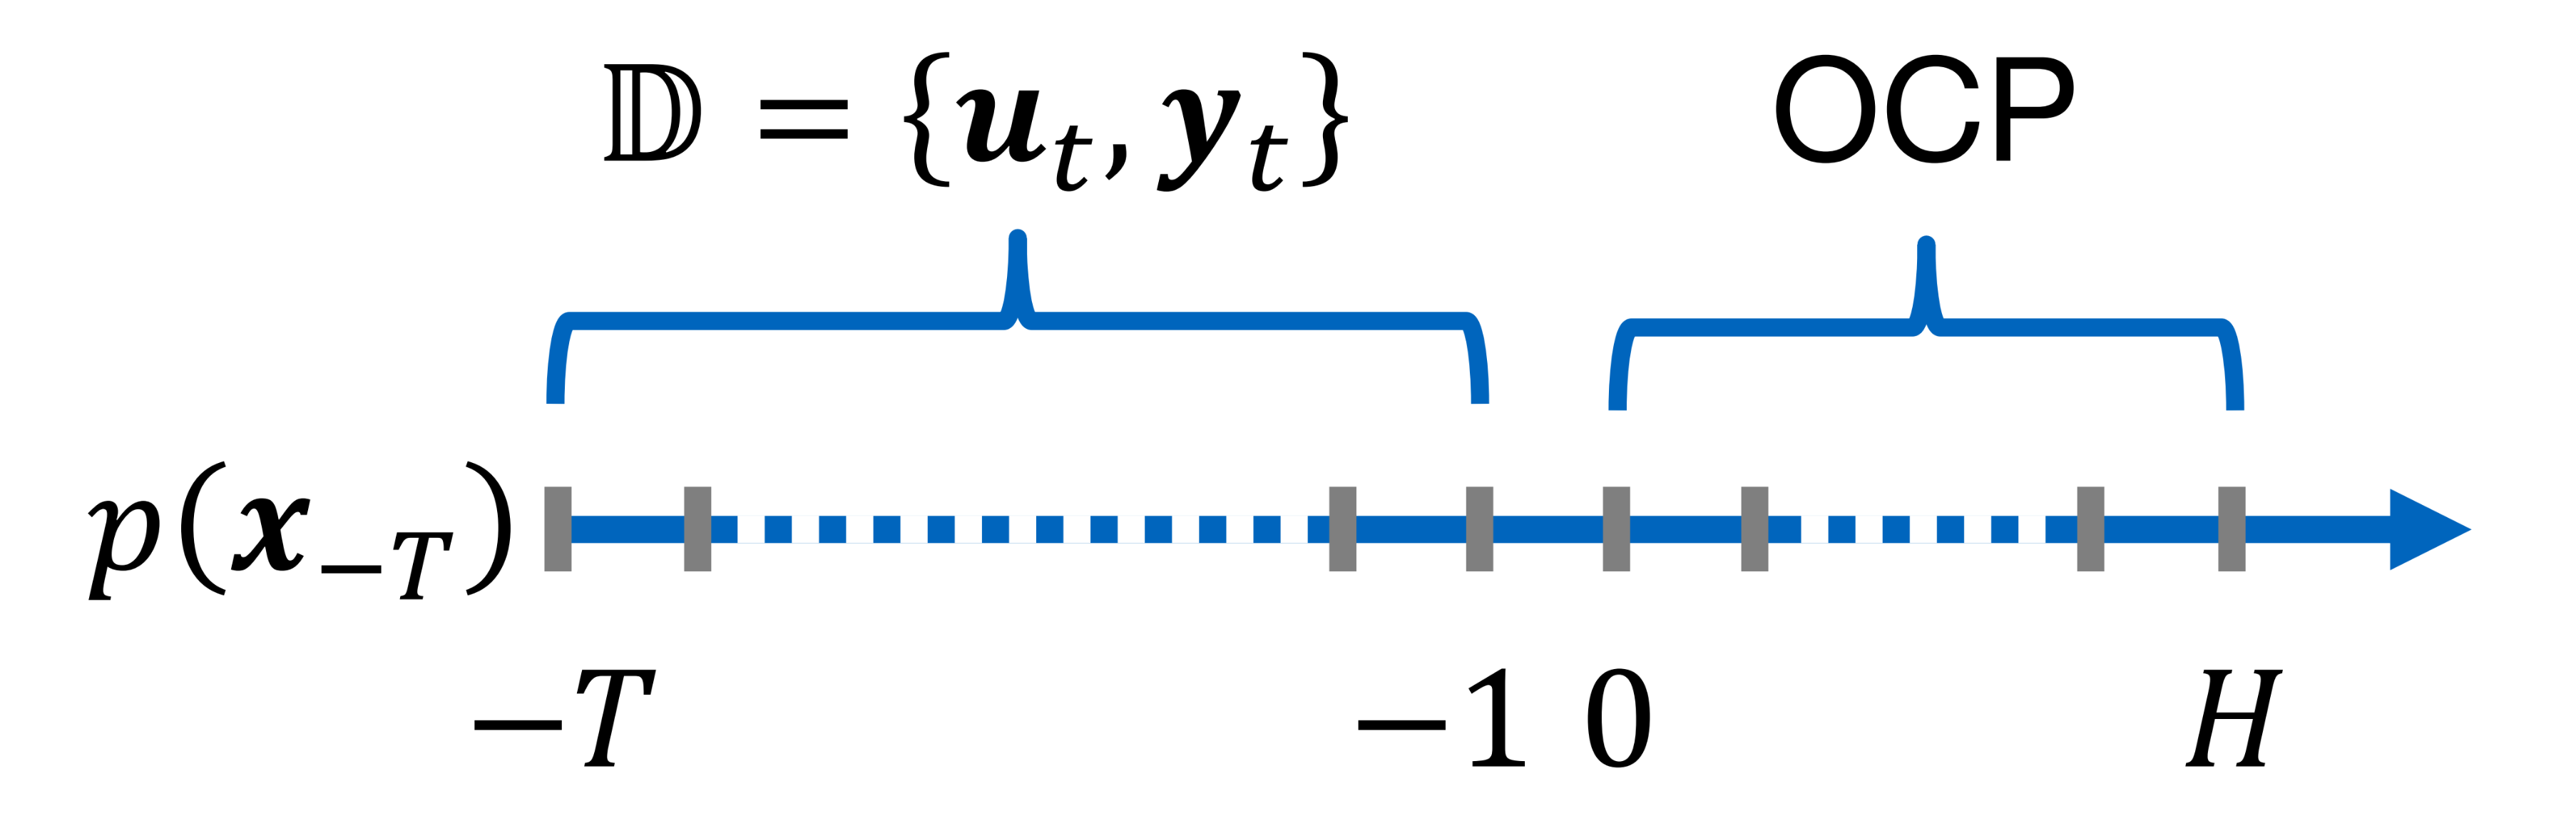
\includegraphics[width= .9\textwidth]{Timeline_pic}
\end{frame}

\begin{frame}{Scenario Generation}
\textbf{Goal:} Generate scenarios $\boldsymbol{\delta}^{[1:N]}$ using the observations $\mathbb{D}$\\
\begin{block}{Algorithm: Scenario Generation}
For $n = 1,...,N$:
\begin{enumerate}
  \item Sample $\{ \boldsymbol{\theta}, \boldsymbol{x}_{\text{-}T:\text{-}1} \}^{[n]}$ from $p\left( \boldsymbol{\theta}, \boldsymbol{x}_{\text{-}T:\text{-}1} \mid \mathbb{D} \right)$ using PMCMC \cite{Robert_24}.
  \item Sample $\boldsymbol{v}_t^{[n]}$ from $\boldsymbol{\mathcal{V}}_{\boldsymbol{\theta}^{[n]}}$ and  $\boldsymbol{w}_t^{[n]}$ from $\boldsymbol{\mathcal{W}}_{\boldsymbol{\theta}^{[n]}}$ for $t = \text{-}1, ..., H$
  \item Set $\boldsymbol{x}_0^{[n]} = \boldsymbol{f}_{\boldsymbol{\theta}^{[n]}} \left( \boldsymbol{x}_{\text{-} 1}^{[n]}, \boldsymbol{u}_{\text{-} 1} \right) + \boldsymbol{v}_{\text{-} 1}^{[n]}$
\end{enumerate}
\textbf{Output:} Scenarios $\boldsymbol{\delta}^{[1:N]} = \{ \boldsymbol{\theta}, \boldsymbol{x}_0, \boldsymbol{v}_{0:H}, \boldsymbol{w}_{0:H}\}^{[1:N]}$
\end{block}
\end{frame}

\begin{frame}{Bootstrap Construction}
\begin{block}{Algorithm: Bootstrap MMD ambiguity set}
\begin{enumerate}
\item $\boldsymbol{K} \leftarrow \textit{kernel}(\boldsymbol{\delta}, \boldsymbol{\delta})$
\item \textbf{For} $m = 1,...,B$
\item \;\; $I \leftarrow N$ numbers from $\{1, \dots N \}$ with replacement
\item \;\; $K_x \leftarrow \sum_{i,j = 1}^N K_{ij}, \;K_y \leftarrow \sum_{i,j \in I} K_{ij}, \;K_{xy} \leftarrow \sum_{j \in I} \sum_{i = 1}^N K_{ij}$
\item \;\; MMD$[m] \leftarrow \frac{1}{N^2} \left( K_x + K_y - 2 K_{xy} \right) $
\item \textbf{End For} 
\item MMD $ \leftarrow$ \textit{sort}(MMD)
\item $\varepsilon \gets$ MMD$\left[ \textit{ceil} (B \beta) \right]$
\end{enumerate}
\textbf{Output:} Gram matrix $\boldsymbol{K}$, Radius of MMD ambiguity set $\varepsilon$
\end{block}
$B = 1000, \beta = 0.95$
\end{frame}



\begin{frame}{Max Constraint}

\begin{block}{Chance Constraint}
	\begin{equation*}
		P \left[ \text{max}(\boldsymbol{h}(\boldsymbol{u}_{0:H},  \boldsymbol{x}_{0:H},  \boldsymbol{y}_{0:H})) \leq 0 \right] \geq 1 - \alpha
	\end{equation*}
\end{block}
			\only<1>{\;\; Constrained Output ($\alpha = 0.5$)
			\begin{figure}
			\pgfplotsset{width=.6\textwidth, compat = 1.18, 
			height = .4\textwidth, grid= major, 
			legend cell align = left, ticklabel style = {font=\scriptsize},
			every axis label/.append style={font=\scriptsize},
			legend style = {font=\scriptsize},
	        }
			\def\file{data/Kernel_K300_Alpha05_S2_MaxConstraint.txt}
			
			\centering
			\begin{tikzpicture}
			\begin{axis}[
			grid=none,
			xmin=0, xmax=40,
			ymin=-14, ymax=14,
			xtick={0, 10, 20, 30, 40},
			ytick={-10, -5, 0, 5, 10},
			ylabel=$y$, xlabel=$t$,
			set layers=standard,
			reverse legend,
			legend style={font=\scriptsize, at={(1,0)},anchor=south east, row sep=2pt},
			ylabel shift = -6 pt]
			
			\addplot[name path=A, forget plot, thick, opacity=0.2] table[x=t,y=y_opt_max]{\file};
			\addplot[name path=B, thick, opacity=0.2] table[x=t,y=y_opt_min]{\file};
			\tikzfillbetween[of=A and B]{opacity=0.2};
			\addlegendentry{$\left\{y_{0:H}^{[1:N]} \right\}$}
			
			\addplot[ultra thick,black!20!green] table[x=t,y=y_pred]{\file};
			\addlegendentry{$\frac{1}{N}\sum\limits_{n=1}^N y_{0:H}^{[n]}$}
			
			\addplot[ultra thick, blue] table[x=t,y=y_true]{\file};
			\addlegendentry{$y_{0:H}$}
			
			\draw [fill=red, fill opacity=0.2,red, opacity=0.2] (10,15) rectangle (20,-10); 
			\draw [fill=red, fill opacity=0.2,red, opacity=0.2] (30,10) rectangle (40,-15); 
			\end{axis}
			\end{tikzpicture}
			\end{figure}}

			\only<2>{\begin{figure}[t]
			\pgfplotsset{width=.75\textwidth, compat = 1.18, 
			height = .41\textwidth, grid= major, 
			legend cell align = left, ticklabel style = {font=\scriptsize},
			every axis label/.append style={font=\scriptsize},
			legend style = {font=\scriptsize},
        }
		\def\file{data/AlphaTest_K300_MaxConstraints_S2_Alpha04.txt}
		
		\centering
		\begin{tikzpicture}
		\begin{axis}[
		grid=both,
		xmin=1, xmax=250,
		ymin=0, ymax=100,
		xtick={0, 50, 100, 150, 200, 250},
		ytick={0, 20, 40, 60, 80, 100},
		ylabel={Constraints Satisfied [\%]}, xlabel=$N$,
		set layers=standard,
		reverse legend,
		legend style={font=\scriptsize, at={(1,0)},anchor=south east, row sep=2pt},
		ylabel shift = -6 pt]
		
		\addplot[ultra thick,black!20!red] table[x=K,y=Kernel04]{\file};
		\addlegendentry{Kernel ($\alpha = 0.4$)}
		
		\addplot[ultra thick,black!20!orange] table[x=K,y=Kernel03]{\file};
		\addlegendentry{Kernel ($\alpha = 0.3$)}

		\addplot[ultra thick,black!20!yellow] table[x=K,y=Kernel02]{\file};
		\addlegendentry{Kernel ($\alpha = 0.2$)}


		\addplot[ultra thick,black!20!blue] table[x=K,y=Scenario]{\file};
		\addlegendentry{Scenario}
		\end{axis}
		\end{tikzpicture}
		\label{fig:robustness_plot}
\end{figure}}
\end{frame}	

\begin{frame}{Maximum Mean Discrepancy (MMD)}
\begin{block}{Maximum Mean Discrepancy}
\begin{equation*}
\begin{aligned}
\text{MMD}(\tilde{P}, P_N) &= ||\mu_{\tilde{P}} - \mu_{P_N} ||_{\mathcal{H}}\\
&= \text{E}_{x,x' \sim \tilde{P}}[k(x,x')] + \text{E}_{y,y' \sim P_N}[k(y,y')] - 2\text{E}_{x\sim \tilde{P}, y \sim P_N}[k(x,y)]
\end{aligned}
\end{equation*}
\end{block}

\begin{block}{(Biased) MMD estimator}
\begin{equation*}
\widehat{\text{MMD}} (P, W) = \frac{1}{N^2} \sum_{i,j = 1}^N k(\boldsymbol{\delta}^{[i]}, \boldsymbol{\delta}^{[j]}) + k(\tilde{\boldsymbol{\delta}}^{[i]}, \tilde{\boldsymbol{\delta}}^{[j]}) - 2 k(\boldsymbol{\delta}^{[i]}, \tilde{\boldsymbol{\delta}}^{[j]})
\end{equation*}
\end{block}

\end{frame}

\end{document}